\documentclass{beamer}

\mode<presentation>
{
  \usetheme{Warsaw}
  \setbeamercovered{transparent}
}

\usepackage[english]{babel}
\usepackage[utf8]{inputenc}
\usepackage{times}
\usepackage[T1]{fontenc}
\usepackage{graphicx}
\graphicspath{ {images/} }


\title[]
{Implementacja wydajnego wzorca wstrzykiwania zależności dla złożonych grafów zależności}

\author[Adrian Mularczyk]
{Adrian Mularczyk}

\institute[Uniwersytet Wrocławski]
{
Uniwersytet Wrocławski\\
Wydział Matematyki i Informatyki\\
Kierunek: Informatyka
}

\date{}

\begin{document}

\begin{frame}
%Nazywa się Adrian Mularczyk i przedstawię Państwu moją pracę magisterską o tytule Implementacja wydajnego wzorca wstrzykiwania zależności dla złożonych grafów zależnoci.
%Praca została napisana pod kierunek Pana doktora Wiktora Zychli.
  \titlepage
 
\begin{small}
\begin{flushright}
Praca wykonana pod kierunkiem dr. Wiktora Zychli
\end{flushright}
\end{small}
 
\end{frame}

\begin{frame}{Agenda}
%Tutaj krótka agenda i czym dzisiaj będę mówił. Najpierw opiszę jaki jest problem. Potem w kilku zdaniach opowiem czym jest wstrzykiwanie zależności, a następnie przejdziemy do mojego rozwiążaniach. Na koniec zaprezentuję niektóre z wyników.
  \tableofcontents
\end{frame}


\section{Przedstawienie problemu}

\begin{frame}{}
%Na przestrzeni lat powstało bardzo dużo projektów. Część z nich była łatwiejsza w utrzymaniu, część trudniejsza. Analiza tych projektów pozwoliła zauważyć, że są pewne zasady, które powodują, że projekty rozwija się łatwiej. Te zasady zostały połączone w zbiory zasad.
\begin{center}
\huge{Przedstawienie problemu}
\end{center}
\end{frame}

\subsection*{SOLID}

\begin{frame}{SOLID}
%Najbardziej popularnych i powszechnie stosowanym zbiorem zasad jest SOLID. Składa się on z pięciu zasady: Single responsibility principle, open/close principle, liskov substituion principle, interface segregation principle oraz dependency inversion principle.
%Niniejsza praca w dużej mierze skupia się na rozwiązaniu ostatniej z tych zasad.
\begin{itemize}
	\item S - SRP (Single responsibility principle)
	\item O - OCP (Open/closed principle)
	\item L - LSP (Liskov substitution principle)
	\item I - ISP (Interface segregation principle)
	\item D - DIP (Dependency inversion principle)
\end{itemize}
\end{frame}

\begin{frame}{Dependency Inversion Principal}
%Dependency Inversion Principal mówi o tym, że wysokopoziomowe moduły nie powinny zależeć od modułów niskopoziomowych. Zależności między nimi powinny wynikać z abstrakcji.
\begin{center}
Dependency Inversion Principal
\end{center}
\end{frame}


\subsection*{Kontenery wstrzykiwania zależności}

\begin{frame}{Kontenery wstrzykiwania zależności}
%Aby łatwiej zastosować przedstawioną zasadę można wesprzeć się tzw. kontenerem wstrzykiwania zależności.
%Taki kontener jest obiektem, który przechowuje mapę, w której abstrakcje (interfejsy, klasy abstrakcyjne) mają przyporządkowane implementacje, czyli klasy implementujące interfejsy lub dziedziczące z klas abstrakcyjnych.
%Kontenery dostarczają nam kilku funkcjonalności.
%Jedną z nich jest możliwość zdefiniowania tego jakiej instancję jakiej klasy należy zwrócić w miejsce konkretnego interfejsu - czyli rejestracja.
%Drugą jest tworzenie instancji obiektów konkretnej klasy lub implementujących określony interfejs.
\begin{itemize}
	\item Rejestracja
	\item Tworzenie obiektów
\end{itemize}
\end{frame}

\subsection*{Obserwacje}

\begin{frame}{Obserwacje}
%Gdy posiadamy już taki kontener, to możemy zauważyć następujące rzeczy:
%W grafach zależności często powtarzają się niektóre typy,
%utworzenie instancji nowego obiektu zajmuje czas,
%a także nowe obiekty są często tworzone.
  \begin{itemize}
  \item W grafach zależności często powtarzają się typy
  \item Utworzenie instancji nowego obiektu zajmuje czas
  \item Nowe obiekty są często tworzone
  \end{itemize}
\end{frame}

\subsection*{Cel Pracy}

\begin{frame}{Cel Pracy}
%I tu przechodzimy do celu mojej pracy, jakim jest stworzenie wydajenego kontenera wstrzykiwania zależności, który będzie wydajny dla zlożonych grafów zależności, a także który będzie efektywnie tworzył kolejne instancje tej samej klasy.
\begin{center}
Wydajeny kontener wstrzykiwania zależności
\end{center}
\end{frame}


\section{Wstrzykiwanie zależności}

\begin{frame}{}
%Wspomniałem o wstrzykiwaniu zależności, ale czym ono jest? Jest to techniką, która umożliwia luźne powiązania, a luźne powiązania sprawiają, że kod jest rozszerzalny i łatwy w utrzymaniu.
\begin{center}
\huge{Wstrzykiwanie zależności}
\end{center}
\end{frame}

\subsection*{Rodzaje wstrzykiwania zależności}

\begin{frame}{Rodzaje wstrzykiwania zależności}
%Wstrzykiwanie zależności może odbywać się na 3 sposoby:
%wstrzykiwanie przez konstruktor, przez metodę oraz przez właściwość
\begin{itemize}
	\item Wstrzykiwanie przez konstruktor
	\item Wstrzykiwanie przez metodę
	\item Wstrzykiwanie przez właściwość
\end{itemize}
\end{frame}


\subsection*{Implementacje przemysłowe}

\begin{frame}{Implementacje przemysłowe}
%Na rynku jest wiele implementacji wstrzykiwania zależności. Poniżej przedstawiono kilka najbardziej popularnych (według ilości pobrań z NuGet) oraz kilka najszybszych (według rankingu na blogu Daniela Palme).
\begin{itemize}
	\item Unity
	\item NInject
	\item Autofac
	\item StructureMap
	\item Windsor
	\item Grace
	\item DryIoc
	\item LightInject
	\item SimpleInjector
\end{itemize}
\end{frame}



\section{Implementacja}

%Wiemy jaki jest problem, to teraz pora opis mojego rozwiązanie. Na początku chciałbym pokrótce opisać dwie rzeczy, które są istotne dla mojego rozwiązania.
\begin{frame}{}
\begin{center}
\huge{Implementacja}
\end{center}
\end{frame}

\begin{frame}{Implementacja}
% Pierwszą z nich jest Common Intermediate Language, w skrócie CIL, a drugą jest przestrzeń nazw Reflection.Emit.
%CIL jest to język pośredni do którego jest kompilowany kod C\#. Język ten pozwala na komunikację między aplikacjami napisanymi na platformie .NET, a systemem operacyjnym. CIL jest językiem w całości opartym na stosie.
%Dodatkowo jest w nim możliwość zdefiniowania zmiennych lokalnych, a także wczytania argumentów. Dostępnymi operacjami są: pobranie wartości ze stosu, umieszczenie wartości na stosie, operacje arytmetyczne oraz wywołanie funkcji.
%Przestrzeń nazw Reflection.Emit pozwala w kodzie programu, w sposób dynamiczny, na utworzenie listy operacji w języku CIL, a następnie zapamiętanie ciągu tych operacji jako funkcji. Za każdym razem, gdy funkcja zostanie wywołana, wykona się ciąg wcześniej zdefiniowanych operacji CIL.
\begin{itemize}
	\item CIL
	\item Reflection.Emit
\end{itemize}
\end{frame}

\subsection*{Dwa rozwiązania}

\begin{frame}{Dwa rozwiązania}
%Jeśli chodzi o moje rozwiązanie, to pomysł był taki, aby wykorzystać Reflection.Emit do utworzenia listę operacji w języku CIL, która dla danego typu, zwróci nam obiekt tego typu.
%Ten pomysł został zrealizowany na dwa sposóby.
%Jedno rozwiązanie nazwałem Partial Emit Function, a drugie Full Emit Function.
%W obu rozwiązaniach metoda do rejestracji wygląda tak samo. Różnią się one jedynie tym jak nowy obiekt jest tworzony.
\begin{itemize}
	\item Partial Emit Function
	\item Full Emit Function
\end{itemize}
\end{frame}


\subsection*{Partial Emit Function}

\begin{frame}{Partial Emit Function}
%Dla tego rozwiązania algorytm działa rekurencyjnie. Dla danego typu najpierw tworzone są obiekty, które są wymagane przez konsruktor tego typu, a następnie nowy obiekt danego typu jest tworzony z wykorzystaniem wcześniej utworzonej listy typów.
%Metoda ta została nazwana Partial, ponieważ obiekt jest tworzony częściowo, kawałek po kawałku, zaczynając od najbardziej skrajnego lewego liścia. Używam tutaj przeszukania w głąb.
%Tworzenie każdego z potrzebnych typów wykorzystuje Reflecion.Emit. Tworzę funkcję, który jako argument przyjmuje listę obiektów wymaganych przez konstruktor danego typu, a następnie przy użyciu tego konstruktora i listy obiektów tworzony jest nowy obiekt. I tak aż do samego korzenia. Czyli jest graf jest złożony, to zostanie wykonany wiele funkcji, które zawierają nieduży ciąg operacji CIL.
\begin{figure}[H]
	\begin{center}
  		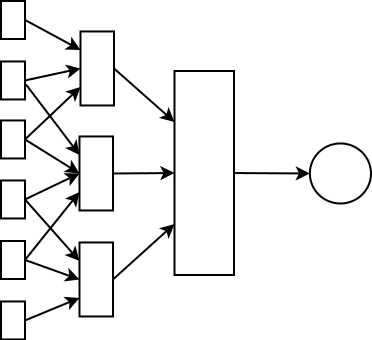
\includegraphics[height=6cm]{PresentationPartial.png}
	\end{center}
\end{figure}
\end{frame}


\subsection*{Full Emit Function}

\begin{frame}{Full Emit Function}
%W tym rozwiązaniu jest tworzona tylko jedna dużą listę operacji CIL. Ta lista zawiera tworzenie wszystkich pośrednich obiektów oraz tworzenie głównego obiektu.
\begin{figure}[H]
	\begin{center}
  		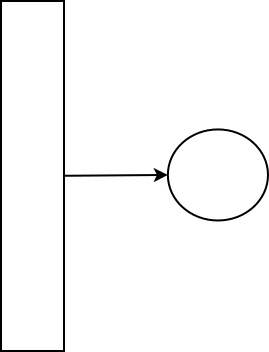
\includegraphics[height=6cm]{PresentationFull.png}
	\end{center}
\end{figure}
\end{frame}




\section{Wyniki}
\begin{frame}{}
%Dlaczego dwa rozwiązania? Ponieważ jak pokazują wyniki czasem bardziej opłąca się używać pierwszego rozwiązania, a czasem drugiego.
%Dodatkowo chciałem się przekonać, czy faktycznie zaprezentowane przeze mnie rozwiązania są wydajne. Porównałem je z przedstawioną wcześniej listą implementacji przemysłowych.
%Jeśli chodzi o testy, to utworzyłem cztery przypadki testowe i dla każdego z nich przeprowadziłem 5 testów - po jednym dla każdego typu rejestracji. Dla każdego z tych testów porównałem osobno czasy dla 1, 10, 100 i 1000 iteracji.
%Tutaj zaprezentuję wyniki tylko dla jednego testu - Transient, który jest najbardziej popularnym typem rejestracji. Przedstawię wyniki tylko dla dwóch przypadków testowych, ponieważ wyniki dla pozostałych dwóch są bardzo zbliżone.
\begin{center}
\huge{Wyniki}
\end{center}
\end{frame}

\subsection*{Przypadek testowy A}

\begin{frame}{Przypadek testowy A - graf zależności}
%W tym teście mamy zdefiniowanych 11 typów. Każdy z nich przyjmuje w konstruktorze o jeden parametr mniej niż typ poprzedni (czyli przyjmują one kolejno od 10 do 0 parametrów w konstruktorze).
%Typ główny, którego instancję będziemy tworzyć przyjmuje wszystkie 10 parametrów. Każdy kolejny typ przyjmuje te same typy co typ poprzedni za wyjątkiem samego siebie. Ostatni typ ma konstruktor bezparametrowy.
%W jednej iteracji jest tworzonych łącznie 1 024 obiektów.
\begin{figure}[H]
	\begin{center}
  		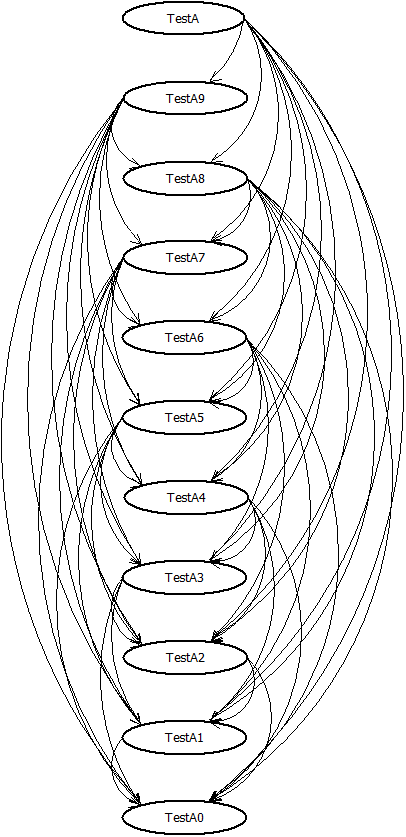
\includegraphics[height=6cm]{TestA.png}
	\end{center}
\end{figure}
\end{frame}

\begin{frame}{Przypadek testowy A - Transient}
%Dla 1 iteracji najniższy czas osiągnął Autofac, ale rozwiązanie Partial osiągnęło czas o niewiele większy. Podobny czas osiągnął również Windsor, a pozostałe rozwiązania mają te czasy już znacząco większe.
%Dla 10 iteracji już rozwiązanie Partial ma najlepszy czas. Jeśli chodzi o rozwiązanie Full, to nie zanotowało ono zauważalnego wzrostu czasu w stosunku do 1 iteracji.
Liczba iteracji: 1 i 10
\begin{table}
\begin{small}
	\begin{tabular}{ l  r }
		\begin{tabular}{ | l | r | }
    		\hline
		Autofac &  0 \\ \hline
		\textbf{NiquIoCPartial}  & \textbf{1} \\ \hline
		Windsor & 1 \\ \hline
		\textbf{NiquIoCFull} & \textbf{8} \\ \hline
		Unity & 8 \\ \hline
		LightInject & 10 \\ \hline
		StructureMap & 10 \\ \hline
		Ninject & 11 \\ \hline
		SimpleInjector & 13 \\ \hline
		DryIoc & 14 \\ \hline
		Grace & 15 \\ \hline
  		\end{tabular}
	&
		\begin{tabular}{ | l | r | }
    		\hline
		\textbf{NiquIoCPartial} & \textbf{3} \\ \hline
		Autofac & 6 \\ \hline
		\textbf{NiquIoCFull} & \textbf{8} \\ \hline
		LightInject & 10 \\ \hline
		SimpleInjector & 14 \\ \hline
		StructureMap & 14 \\ \hline
		DryIoc & 15 \\ \hline
		Grace & 16 \\ \hline
		Unity & 16 \\ \hline
		Windsor & 16 \\ \hline
		Ninject & 90 \\ \hline
  		\end{tabular}
  	\end{tabular}
\end{small}
\end{table}
\end{frame}


\begin{frame}{Przypadek testowy A - Transient}
%Dla 100 iteracji można zaobserwować, że rozwiązanie Full nadal ma niewielki wzrost czasu w stosunku do znaczącego wzrostu liczby iteracji. Ten wzrost jest natomiast zauważalny dla rozwiązania Partial i wszystkie z rozwiązań, które są uważąne za najszybsze zanotowały lepszy czas do niego. Jednakże rozwiązanie Partial wciąż zanotowało czasy znacząco lepsze niż wszystkie najpopularniejsze rozwiązania.
%Dla 1000 iteracji niewiele się zmieniło jeśli chodzi o pozycje, ale można zaobserwować, że pierwsze 5 rozwiązań na wzrost około 2-krotny, a pozostałe 6 rozwiązań około 10-krotny.
Liczba iteracji: 100 i 1000
\begin{table}
\begin{small}
	\begin{tabular}{ l  r }
		\begin{tabular}{ | l | r | }
    		\hline
		\textbf{NiquIoCFull} & \textbf{9} \\ \hline
		LightInject & 11 \\ \hline
		SimpleInjector & 15 \\ \hline
		DryIoc & 16 \\ \hline
		Grace & 18 \\ \hline
		\textbf{NiquIoCPartial} & \textbf{19} \\ \hline
		StructureMap & 54 \\ \hline
		Autofac & 59 \\ \hline
		Unity & 88 \\ \hline
		Windsor & 155 \\ \hline
		Ninject & 882 \\ \hline
  		\end{tabular}
	&
		\begin{tabular}{ | l | r | }
    		\hline
		\textbf{NiquIoCFull} & \textbf{18} \\ \hline
		LightInject & 19 \\ \hline
		SimpleInjector & 29 \\ \hline
		DryIoc & 29 \\ \hline
		Grace & 37 \\ \hline
		\textbf{NiquIoCPartial} & \textbf{173} \\ \hline
		StructureMap & 417 \\ \hline
		Autofac & 587 \\ \hline
		Unity & 813 \\ \hline
		Windsor & 1529 \\ \hline
		Ninject & 8934 \\ \hline
  		\end{tabular}
  	\end{tabular}
\end{small}
\end{table}
\end{frame}


\subsection*{Przypadek testowy C}

\begin{frame}{Przypadek testowy C - graf zależności}
%Dla tego przypadku testowego graf zależności wygląda zupełnie inaczej. Jest tutaj zdefiniowanych 26 typów. 5 z tych typów ma konstruktor bezparametrowy, a pozostałe 21 ma konstruktor z pięcioma parametrami.
%Za wyjątkiem pierwszych 6 typaów, każdy typ występuje w 5 konstruktorach.
%Tutaj w 1 iteracji jest tworzonych prawie 4 tysiące obiektów (3 906 obiektów).
\begin{figure}[H]
	\begin{center}
  		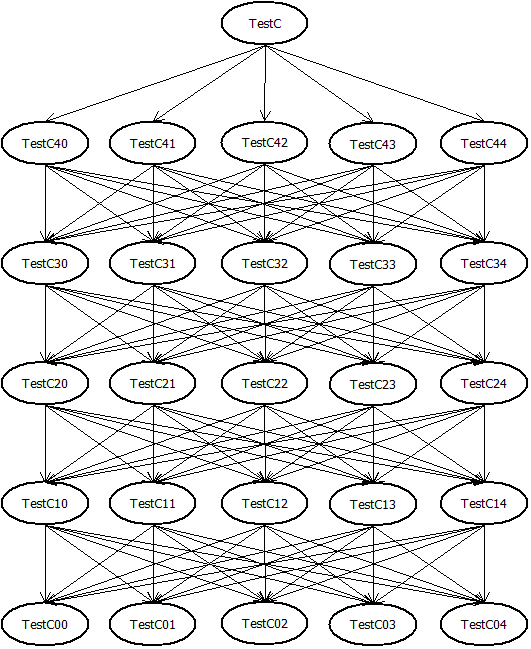
\includegraphics[height=6cm]{TestC.png}
	\end{center}
\end{figure}
\end{frame}

\begin{frame}{Przypadek testowy C - Transient}
%Dla 1 iteracji te same rozwiązania mają najlepsze czasy, czyli Autofac, Partial oraz Windsor.
%Dla 10 iteracji układ tabeli jest bardzo zbliżony do poprzedniego przypadku. Ponownie najlepiej radzi sobie rozwiązanie Partial, a rozwiązanie Full zaczyna mieć lepsze czasy od pozostałych rozwiązań.
Liczba iteracji: 1 i 10
\begin{table}
\begin{small}
	\begin{tabular}{ l  r }
		\begin{tabular}{ | l | r | }
    		\hline
		Autofac & 2 \\ \hline
		\textbf{NiquIoCPartial} & \textbf{4} \\ \hline
		Windsor & 7 \\ \hline
		Unity & 19 \\ \hline
		StructureMap & 26 \\ \hline
		\textbf{NiquIoCFull} & \textbf{31} \\ \hline
		LightInject & 36 \\ \hline
		DryIoc & 39 \\ \hline
		Ninject & 39 \\ \hline
		SimpleInjector & 41 \\ \hline
		Grace & 61 \\ \hline
  		\end{tabular}
	&
		\begin{tabular}{ | l | r | }
    		\hline
		\textbf{NiquIoCPartial} & \textbf{10 }\\ \hline
		Autofac & 24 \\ \hline
		\textbf{NiquIoCFull} & \textbf{32} \\ \hline
		LightInject & 37 \\ \hline
		DryIoc & 40 \\ \hline
		StructureMap & 40 \\ \hline
		SimpleInjector & 41 \\ \hline
		Unity & 47 \\ \hline
		Grace & 62 \\ \hline
		Windsor & 62 \\ \hline
		Ninject & 353 \\ \hline
  		\end{tabular}
  	\end{tabular}
\end{small}
\end{table}
\end{frame}


\begin{frame}{Przypadek testowy C - Transient}
%Dla 100 i 1000 iteracji tym razem układ również jest zbliżony do poprzedniego przypadku testowego, czyli najlepszy czas ma rozwiązanie Full, następnie szybkie rozwiążania, a dalej rozwiązanie Partial.
%Tutaj również dla pierwszych 5 rozwiązań wzrost jest 2-krotny, a pozostały 6 około 10-krotny.
Liczba iteracji: 100 i 1000
\begin{table}
\begin{small}
	\begin{tabular}{ l  r }
		\begin{tabular}{ | l | r | }
    		\hline
		\textbf{NiquIoCFull} & \textbf{38} \\ \hline
		LightInject & 44 \\ \hline
		DryIoc & 47 \\ \hline
		SimpleInjector & 49 \\ \hline
		Grace & 73 \\ \hline
		\textbf{NiquIoCPartial} & \textbf{74} \\ \hline
		StructureMap & 181 \\ \hline
		Autofac & 231 \\ \hline
		Unity & 318 \\ \hline
		Windsor & 608 \\ \hline
		Ninject & 3511 \\ \hline
  		\end{tabular}
	&
		\begin{tabular}{ | l | r | }
    		\hline
		\textbf{NiquIoCFull} & \textbf{82} \\ \hline
		LightInject & 86 \\ \hline
		DryIoc & 99 \\ \hline
		SimpleInjector & 116 \\ \hline
		Grace & 155 \\ \hline
		\textbf{NiquIoCPartial} & \textbf{690} \\ \hline
		StructureMap & 1540 \\ \hline
		Autofac & 2288 \\ \hline
		Unity & 3015 \\ \hline
		Windsor & 6037 \\ \hline
		Ninject & 37642 \\ \hline
  		\end{tabular}
  	\end{tabular}
\end{small}
\end{table}
\end{frame}


\section{Podsumowanie}

\begin{frame}{}
%Jak można było zobaczyć na zarezentowanych wynikach, moje rozwiązania bardzo dobrze realizują postawione we wstępie pracy cele. Dla wszystkich przypadków testowych, dla każdego z rodzaju rejestracji, albo jedno z moich rozwiązań osiągęło najlepszy wyniki albo jego wyniki niewiele odbiegał od najlepszego wyniku. Zawsze któreś z moich rozwiązań było w pierwszej trójce rozwiązań z najlepszymi czasami, a czasami nawet oba. Cowięcej moje rozwiązania można mieszać, czyli w jednym projekcie można korzystać z obu rozwiązań niezależnie. Dzięki temu patrząc całościowo, to moje rozwiązanie jest najbardziej wydajną implementacją wzorca wstrzykiwania zależności dla złożonych grafów zależności.
%Dziękuję.
\begin{center}
\huge{Podsumowanie}
\end{center}
\end{frame}

\end{document}


